\documentclass[letterpaper,10pt]{article}

\usepackage{titling}
\usepackage{listings}
\usepackage{url}
\usepackage{setspace}
\usepackage{subfig}
\usepackage{sectsty}
\usepackage{pdfpages}
\usepackage{colortbl}
\usepackage{multirow}
\usepackage{relsize}
\usepackage{amsmath}
\usepackage{fancyvrb}
\usepackage{amsmath,amssymb,amsthm,graphicx,xspace}
\usepackage[titlenotnumbered,noend,noline]{algorithm2e}
\usepackage[compact]{titlesec}
\usepackage[default]{droidserif}
\usepackage[T1]{fontenc}
\usepackage{tikz}
\usetikzlibrary{arrows,automata,shapes,trees,matrix,chains,scopes,positioning,calc}
\tikzstyle{block} = [rectangle, draw, fill=blue!20, 
    text width=2.5em, text centered, rounded corners, minimum height=2em]
\tikzstyle{bw} = [rectangle, draw, fill=blue!20, 
    text width=4em, text centered, rounded corners, minimum height=2em]

\definecolor{namerow}{cmyk}{.40,.40,.40,.40}
\definecolor{namecol}{cmyk}{.40,.40,.40,.40}

\let\LaTeXtitle\title
\renewcommand{\title}[1]{\LaTeXtitle{\textsf{#1}}}


\newcommand{\handout}[5]{
  \noindent
  \begin{center}
  \framebox{
    \vbox{
      \hbox to 5.78in { {\bf ECE155: Engineering Design with Embedded Systems } \hfill #2 }
      \vspace{4mm}
      \hbox to 5.78in { {\Large \hfill #4  \hfill} }
      \vspace{2mm}
      \hbox to 5.78in { {\em #3 \hfill} }
    }
  }
  \end{center}
  \vspace*{4mm}
}

\newcommand{\lecture}[3]{\handout{#1}{#2}{#3}{Lecture #1}}
\newcommand{\tuple}[1]{\ensuremath{\left\langle #1 \right\rangle}\xspace}

\addtolength{\oddsidemargin}{-1.000in}
\addtolength{\evensidemargin}{-0.500in}
\addtolength{\textwidth}{2.0in}
\addtolength{\topmargin}{-1.000in}
\addtolength{\textheight}{1.75in}
\addtolength{\parskip}{\baselineskip}
\setlength{\parindent}{0in}
\renewcommand{\baselinestretch}{1.5}
\newcommand{\term}{Spring 2014}

\singlespace


\begin{document}

\lecture{ 26 --- Refactoring}{\term}{Patrick Lam \& Jeff Zarnett}


\section*{Refactoring}
We've repeatedly mentioned the existence of refactoring, especially
when talking about Agile methods. \emph{Refactoring} incrementally
improves code quality using local, semantics-preserving changes to the
code. Our reference in most of this is the definitive reference \cite{fowler}.

Some people believe that for this to count as a refactoring, it has to make the code clearer. You can make lots of changes to your software that have no impact on its semantics (behaviour), but it is only refactoring if it makes the code easier to understand \cite{sourcemaking}. However, ease of understanding is not the only goal, and in this course we will use the more inclusive definition.

Contrast this against performance optimizations: performance optimizations should not change the semantics of the code (just its execution speed), but they may make the code that much harder to understand.

Let's unpack the definitions of the terms we used to define refactoring.

\begin{itemize}
\item {\bf Local}: Refactoring should not affect unrelated parts of the
program; it should only change the parts of the program that you're 
refactoring. When you commit a refactoring to the repository,
you should be sure to only commit the source files that got refactored.
\item {\bf Semantics-preserving}: This means that the behaviour
of the refactored code should be identical to the behaviour of the
original code. If some tool did the refactoring, you can usually be sure
that it was semantics-preserving. Otherwise, your unit tests will help
ensure that you didn't change anything.
\end{itemize}

\subsection*{Motivation}

The first major reason is to improve the design of the software. Nobody gets designs 100\% right on the first try, so you will always find some changes to make. We take the code that is in one structure and we make some changes to create a new (better) structure for it. 

Related to improving the design is the idea of maintaining the design. As programmers change the code, the structure tends to decay. Changes are introduced that break the structure rules or bend things out of place, or are just bolted on where they do not belong \cite{sourcemaking}. If we consistently maintain the structure of the code, it is much easier to preserve. An analogy that students probably have a lot of experience with: when there is one dish to clean in the sink, cleaning it is easy. If the sink is overflowing with dirty dishes then washing them is much more of a chore. When we refactor, we tidy things up (do the dishes) and prevents the work from getting out of hand.

It also make code easier to change. Poorly designed code usually takes more lines to do the work, because code has been copy-and-pasted around. If we change one section but not another, then the behaviour of the software is inconsistent. We can prevent some future errors if the code is easily maintained.

And finally, it makes the code to understand. Someone else is going to need to read the code and make changes. Code that is clearer might take a few more CPU cycles to execute, but it could save that other programmer a week of work in understanding it. This is true even if there are no other programmers working on your code base: yourself a year from now is ``someone else'' who will need to read the code and change it \cite{sourcemaking}. 


\subsection*{Types of Refactoring} The Fowler book classifies the
refactorings into the following broad categories:

\begin{itemize}
\item Composing methods: change what code belongs to which method;
\item Moving features between objects: put fields, methods, classes in
different places;
\item Organizing data: change how data gets stored in your program;
\item Simplifying conditionals: make your {\tt if} statements easier
to understand;
\item Making method calls simpler: change how methods relate to each other;
\item Generalizations: like moving features between objects, but related
to the inheritance hierarchy.
\end{itemize}

\subsection*{Refactoring Algorithm}
The basic pattern for refactoring looks something like this:

\begin{enumerate}
	\item Create unit tests (if needed)
	\item Run unit tests
	\item Make changes
	\item Re-run unit tests
	\item Evaluate results
\end{enumerate}

Hopefully, you already have unit tests so you can skip step one. Then you will run your tests and be sure you are starting from a state where everything is working. Make your changes, and re-run the tests. If the tests fail, then we did not make a semantic-preserving change, and we need to undo some changes and try again.


\subsection*{Examples}
We'll continue by looking at two examples of refactorings this time.
Next time, we'll look at a list of refactorings and talk about refactorings in
general.

\paragraph{Example: Extract Method.} A popular example of a refactoring
is the ``extract method'' refactoring, which splits out part of a
method into an independent method. For instance~\cite{ref:extmeth}:

{\tt
\begin{verbatim}[language=Java]
// (1) make sure the code only runs on mac os x
boolean mrjVersionExists = System.getProperty("mrj.version") != null;
boolean osNameExists = System.getProperty("os.name").startsWith("Mac OS");

if ( !mrjVersionExists || !osNameExists)
{
  System.err.println("Not running on a Mac OS X system.");
  System.exit(1);
}

// (2, 3) do all the preferences stuff, and get the default color
preferences = Preferences.userNodeForPackage(this.getClass());
int r = preferences.getInt(CURTAIN_R, 0);
int g = preferences.getInt(CURTAIN_G, 0);
int b = preferences.getInt(CURTAIN_B, 0);
int a = preferences.getInt(CURTAIN_A, 255);
currentColor = new Color(r,g,b,a);
\end{verbatim}
}

We can instead split this into three sub-methods, which each make more
sense as an independent unit rather than agglomerated into one method:

{\tt
\begin{verbatim}[language=Java]
  dieIfNotRunningOnMacOsX();
  connectToPreferences();
  getDefaultColor();
\end{verbatim}
}

This is particularly useful when the code does the same thing 
many times (``code clones''); you can replace all of the clones with
a call to a single method, which means that you only need to change the
code once. 

A method should have unity of purpose: it should do one
conceptual thing. A good test is that you should be able to come up
with a meaningful name for the method. Note that we are putting some
design into the code through this refactoring.

Although the example here replaces all of the code with method calls,
it's also common to pick out just part of a method and make a separate
function from that, while leaving the rest of the method in
place. Many IDEs support this sort of refactoring with one click.

\paragraph{Another example: Replace Magic Number With Symbolic Constant.}
Here's another example of a refactoring, which is quite applicable to
your labs. Using symbolic constants is often better coding practice
than putting numbers directly into the code. Consider this example~\cite{ref:repconst}:

{\tt
\begin{verbatim}[language=Java]
	double potentialEnergy(double mass, double height) {
		return mass * height * 9.81;
	}
\end{verbatim}}

You can refactor this to:
{\tt \begin{verbatim}[language=Java]
	double potentialEnergy(double mass, double height) {
		return mass * GRAVITATIONAL_CONSTANT * height;
	}
	static final double GRAVITATIONAL_CONSTANT = 9.81;
\end{verbatim}}
\vspace{-1em}
There are two benefits to this refactoring: 1) the refactored code is
easier to understand; and 2) if you might need to change the value of 
the constant, it's easier to do so in one place only.
\vspace{-1em}

\paragraph{When to Refactor} A key decision we will have to make in our software is when it is the right time to refactor. All the options below have advantages and disadvantages. We can use one, a few, or all of them in the same project.

\begin{itemize}
	\item \textbf{Continuously}?\\
	Refactoring done continuously helps prevent the ``pile of dirty dishes'' problem, but it can lead to spending too much time tinkering with the refactoring and not implementing the code. 
	\item \textbf{Fixed Schedule}?\\
	If we refactor on a fixed schedule, say, every three months, that allows us to take some time and examine the code and do a lot of refactorings all at once. 
	\item \textbf{When Fixing a Bug}?\\
	Some advocate for making changes while we fix bugs: if we notice something when we're re-examining code, we fix it right away. However, this strategy is dangerous because it conflates the bug fix with the structural change. 
	\item \textbf{At the End of a Project}?\\
	In other cases, it's desirable to refactor once the code for a project is complete (before it goes into maintenance mode). 
	\item \textbf{At the Start of a Project}?\\
	Lastly, we might consider refactoring at the start of a project; before we open up the module and begin to make our changes and additions, we clean up the code and then begin the new project.
\end{itemize}

\subsection*{List of Refactorings} 

I've augmented Wikipedia's 
non-exhaustive list of
refactorings~\cite{wiki:refactoring}. These refactorings are organized differently 
than the list you saw last time.

\begin{itemize}
\item Techniques that allow for more abstraction:
\begin{itemize}
\item \emph{Encapsulate Field}: force code to access the field with getter and setter methods.
\item \emph{Generalize Type}: create more general types to allow for more code sharing.
\item \emph{Replace conditional with polymorphism}: use inheritance and virtual dispatch instead of a conditional.
\end{itemize}
\item Techniques for breaking code apart into more logical pieces:
\begin{itemize}
\item \emph{Extract Method}: as seen above, pull out part of a larger method into a new method.
\item \emph{Extract Class}: moves code from an existing class into a new class.
\end{itemize}
\item Techniques for integrating code that's needlessly spread apart:
\begin{itemize}
\item \emph{Inline Method}: integrate a copy of the body of a method into its calling method.
\item \emph{Inline Class}: put all of the fields and methods of a class into another class and erase the original.
\end{itemize}
\item Techniques for improving names and location of code:
\begin{itemize}
\item \emph{Move Method/Field}: move to a more appropriate class or source file.
\item \emph{Rename Method/Field}: changing the name into a new one that better reveals its purpose.
\item \emph{Pull Up}: in OOP, move to a superclass.
\item \emph{Push Down}: in OOP, move to a subclass.
\end{itemize}
\end{itemize}

\subsection*{Design Antipatterns}
An antipattern is kind of like antimatter - the opposite of normal matter, and very dangerous. In the context of software development, it is a way of developing your code that is messy or makes errors more likely. Antipatterns are not restricted to software development; there are many of them related to project management. However, when we encounter antipatterns in software, that is something we can often fix with refactoring. From \cite{sourcemaking}, some common antipatterns and suggestions about how to deal with them.


\paragraph{The Blob.}
One object is not only the most important class in the system... it does basically everything. It's called the Blob because of the old horror movie where the alien blob just keeps growing and growing, until it's dangerously large and threatening the entire planet. A Blob design has far too much of the code and logic centralized in one specific class. The solution is to refactor the design to extract methods and classes so that responsibilities are properly distributed. 


\paragraph{Lava Flow.}
Dead code and forgotten design information is frozen in an ever-changing design. A piece code was written by previous developers or just so long ago that everyone forgot, and nobody wants to touch it or delete it for fear of breaking something. It gets the name from the geological phenomenon: lava flows when it is hot, but it cools and hardens into solid rock. These are serious drains on productivity because developers spend time compiling, testing, and refactoring code that is useless. To solve this, identify this dead code (try using ``References'' in Eclipse) and delete it. If it was really important, your unit tests will alert you (and not just the test class for the method or class you deleted). If it turns out it wasn't dead code, just restore an older version from version control.

\paragraph{Functional Decomposition.}
This antipattern is the output of experienced, non-object-oriented developers who design and implement an application in an object-oriented language. The resulting code resembles a structural language (Pascal, FORTRAN) in class structure. It can be incredibly complex as smart procedural developers devise very ``clever'' ways to replicate their time-tested methods in an object-oriented architecture. To solve this, extract classes, merge duplicate code, and create methods such that there is defined structure in the program.

\paragraph{Copy-and-Paste Programming.}
Code reused by copying and pasting lines leads to serious maintenance problems. You may have two methods which are very similar or identical. The solution: extract common elements and make them generic (where applicable). 

\paragraph{Poltergeists.}
Poltergeists are classes with very limited roles and effective life cycles. A poltergeist is the term for a ghost that allegedly causes noise (knocking on a door) or destruction (smashing a lamp). In the context of software, they are objects that pop in, do one thing, then vanish. These are bad design because they are unnecessary and waste resources when they appear and disappear. To get rid of them, we call the Ghostbusters (``Who you gonna call?!''). No, we actually get rid of them by inlining their functionality into other objects.


\paragraph{Golden Hammer.}
The saying is ``When all you have is hammer, everything looks like a nail.''. A Golden Hammer is a familiar technology or concept applied obsessively to many software problems. A hammer is great at what it does, but it's not the solution to every problem. Having a specific architecture, like client-server, is good, but not every problem should be solved that way. To solve this, refactor the code to a more appropriate architecture or design.

\paragraph{Exceptions as Control Flow.}
Exceptions should be, well, exceptions, and they should not be things we normally expect to happen. Using an Exception as part of the normal flow of the program instead of calling the appropriate methods is just bad design. Exceptions are expensive to generate, send, and deal with (and potentially fatal to the execution of your program). Using them for normal operations is rare, and much more common is using them for error handling control flow inappropriately. Instead of having a try-catch block where the catch block does something, refactor this so the condition is checked in advance and the exception is prevented.


\paragraph{Spaghetti Code.}
This is the most famous of all the design antipatterns. It refers to a program that contains little or no structure; there are typically a small number of objects with methods that are really long. Ad-hoc software structure makes it difficult to extend and optimize code. All the refactoring techniques above can be used to deal with different areas, until some structure is formed.


\subsection*{More Refactoring Examples} 
\vspace{-1.5em}
We'll continue by talking about the
refactorings in more detail; perhaps this will help you understand the
goals of refactoring, so that you can do it in your own code.

\paragraph{Encapsulate field.} A common Java idiom is to have private fields,
public accessor methods, and replace all field reads {\tt x.foo} and
writes {\tt x.foo = y}, respectively, with calls to {\tt x.getFoo()}
and {\tt x.setFoo(y)}. The goal of this refactoring is to enhance the modularity of the code. Only the class that defines {\tt x} is allowed to read or write {\tt x}
directly. 

One implication is that you can change the way you store the internal
data inside a class, and it won't affect any other classes. For instance,
you can have a {\tt Point} class which you initially implement using 
x/y coordinates, and then transparently change it to using polar
coordinates without having to change any of the users of the {\tt Point}. 

Not every field needs to be encapsulated, though. For instance, if you 
have a class which represents an RGB colour, it's probably OK to have 
public fields for the red, green and blue fields.


\paragraph{Pull Up Method.} This is an example of a 
generalization. Consider the following UML class diagrams~\cite{ref:pullup}:

\begin{center}
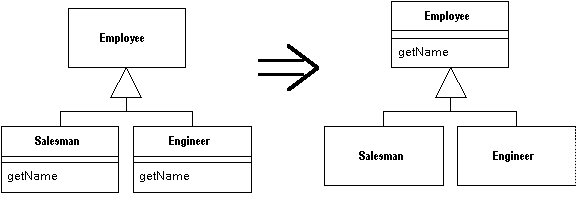
\includegraphics[width=\textwidth]{images/pullUpMethod.png}
\end{center}

What we can see here is that the two subclasses {\tt Salesman} and
{\tt Engineer} both have a common method {\tt getName}, with
identical behaviour. It makes sense to move the method to the common
superclass {\tt Employee}.

\paragraph{Push Down Method.} Conversely, sometimes it makes sense
to push methods down to subclasses~\cite{ref:pushdown}:

\begin{center}
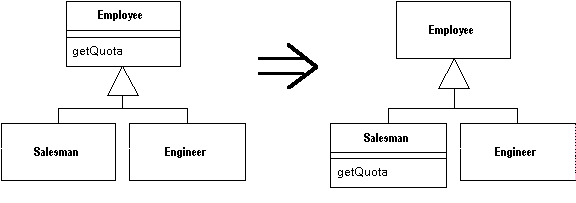
\includegraphics[width=\textwidth]{images/pushDownMethod.png}
\end{center}

In this case, the original design was flawed: {\tt Engineer}s don't
have quotas, only {\tt Salesman}. So we improve the design by 
putting {\tt getQuota} where it should be.

I didn't show you the code, only the UML, but the transformation to the
code should be obvious. Note that in both cases, it's not supposed
to change the behaviour of the program, only improve its design.

\paragraph{Inline Class.} Here's one more refactoring example~\cite{ref:inline}. In this case, we get
rid of helper classes that aren't that useful.

\begin{center}
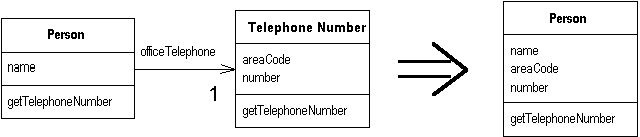
\includegraphics[width=\textwidth]{images/inlineClass.png}
\end{center}

The UML transformation corresponds to a code transformation where we
fold the {\tt areaCode} and {\tt number} fields, along with the
{\tt getTelephoneNumber} method, into the containing {\tt Person} class.
Maybe we found that no one else was using the {\tt Telephone Number} class.
Be sure to delete the class after you've inlined it.

\paragraph{Fix an Antipattern: Exceptions as Control Flow}
In this one, we'll rewrite some code (not using an official, named refactoring), to stop employing the antipattern of exceptions as control flow.

\begin{verbatim}[language={Java}]
try {
   fileReader.readFile(fileSelector.getSelection().getFileName());
} catch (NullPointerException npe) {
   showErrorDialog(Error.NO_FILE_SELECTED);
   return;
}
\end{verbatim} 

The \texttt{NullPointerException} can occur if the selection of the \texttt{fileSelector} is \texttt{null}: we try to call \texttt{getFileName()} on the \texttt{null} resulting in the exception. Now let's rewrite this so that we stop using the Exception handling:

\begin{verbatim}[language={Java}]
if (fileSelector.getSelection() == null) {
   showErrorDialog(Error.NO_FILE_SELECTED);
   return;
}
fileReader.readFile(fileSelector.getSelection().getFileName());
\end{verbatim} 

The functionality of the code is unchanged, but this will be both a performance and readability enhancement.



\bibliographystyle{alpha}
\bibliography{155}


\end{document}
